
% this file is called up by thesis.tex
% content in this file will be fed into the main document

%------------------------------------------------------------------------- 

\chapter{Introducción}
\label{cha:Introduccion}
\lhead{Introducción} % This is for the header on each page - perhaps a shortened title
\graphicspath{{Figures/intro_img/}{../Figures/intro_img/}}

Como es bien sabido, la luz transporta energía; esto se evidencia al
comparar las temperaturas en el día y en la noche o al iluminar una celda
fotovoltáica. En su representación cuántica, la luz está
compuesta por partículas sin masa llamadas fotones. Al no tener masa,
su energía está directamente asociada a su momento, y el momento de 
los fotones así como el de otras partículas en la mecánica cuántica puede ser tanto
lineal como angular. El momento angular se compone a su vez de dos
contribuciones, la de spin y la orbital. Desde un punto de vista 
macroscópico, el momento angular de spin se asocia con la polarización
de la luz, es decir con la dirección de oscilación de los campos
eléctrico y magnético con respecto a un eje coordenado. Asimismo, el
\textbf{momento angular orbital} (\acrshort{OAM}) se asocia con las distribuciones
espaciales de la amplitud y la fase, tal y como se observan
en un plano perpendicular a la propagación de la luz. Para aclarar esta idea
comparemos dos haces polarizados linealmente, uno con OAM
cero, y el otro con OAM +1. El haz de luz que carece de momento
angular orbital presenta una distribución de fase constante. Si éste tiene una distribución de amplitud
Gaussiana, al ser enfocado por una lente, en un plano de
observación veremos que la distribución de intensidad está dada por una función de
Airy como la que se ilustra en la Fig.~\ref{fig:oam_intro}c). 
%\ref{fig:oam0intro}  
%\begin{figure}[h!]
%\centering
%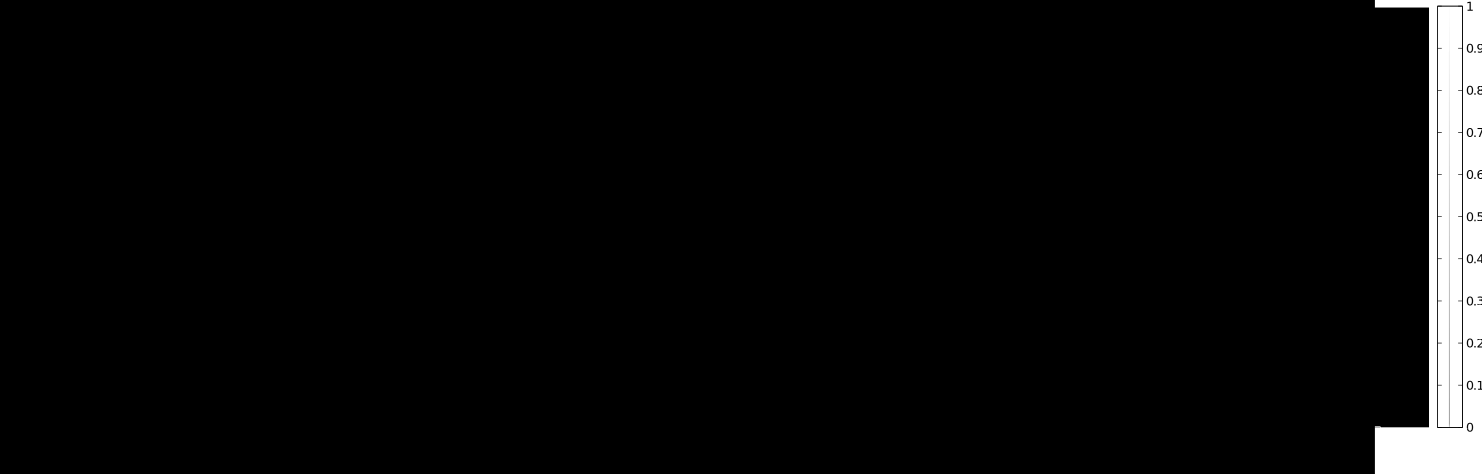
\includegraphics[scale=.33]{img/oam0Intro}
%\caption{a) Amplitud normalizada de un haz plano circular con OAM 0. b)
%Mapa de fase envuelta de $-\pi$ a $\pi$ radianes del mismo haz. c)
%Intensidad normalizada y corte transversal de un haz Gaussiano luego de
%ser enfocado.}
%\label{fig:oam0intro}
%\end{figure}
Por el contrario, el haz con OAM +1 posee una distribución
 de fase helicoidal donde el valor de la fase varía azimutalmente
 desde $\pi$ a $-\pi$ radianes como se muestra  
en la Fig.~\ref{fig:oam_intro}b). Haces con distribuciones de fase de este tipo poseen una
indeterminación de la fase en el centro dado que en la
coordenada $r=0$ confluyen fotones con todos los valores posibles de fase. La
consecuencia directa de la indeterminación en este tipo de puntos es
la ausencia de luz por efecto de superposición. Si, como en el caso
anterior, observamos la intensidad en un plano de enfoque veremos un
perfil con forma de dona como la de la Fig.~\ref{fig:oam_intro} d). 
\begin{figure}[h!]
\centering
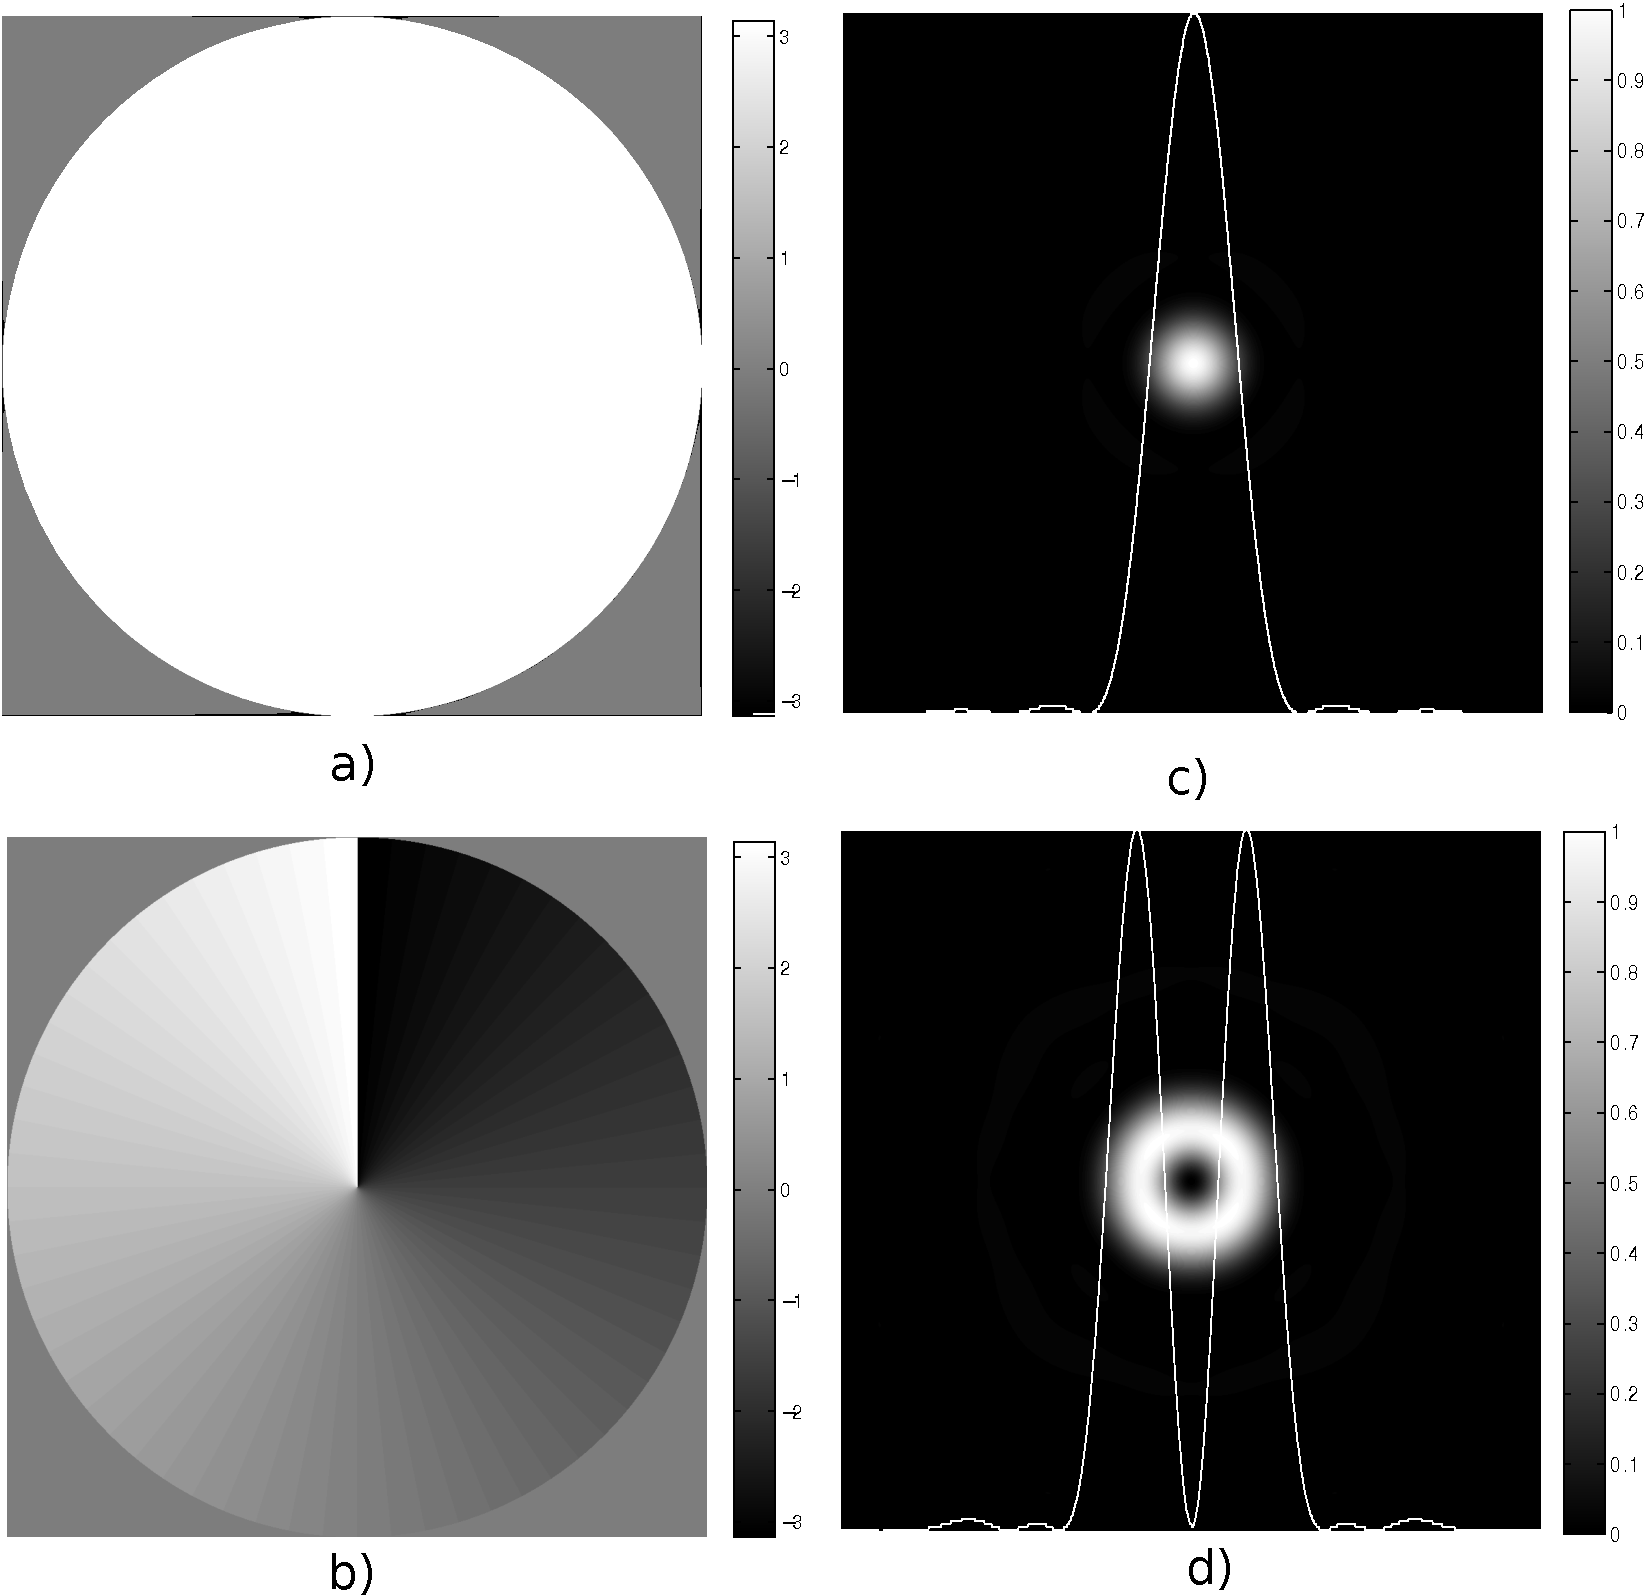
\includegraphics[scale=.33]{oam_Intro}
\caption[Comparación entre haces Gaussianos y haces Laguerre-Gauss]{ Las figuras a) y b) representan mapas de fase de haces con
  OAM 0 y +1 definidos en el intervalo $[- 
  \pi,\pi]$ . Las intensidades correspondientes luego de enfocar los haces en
  un plano de observación se muestran en las figuras c) y d).}
\label{fig:oam_intro}
\end{figure}

Por su naturaleza rotacional, los puntos alrededor de los cuales la fase
varía de $-\pi$  a $\pi$ se conocen como \textbf{vórtices ópticos} (\acrshort{VOs}), y
están presentes siempre que haya haces con momento angular 
orbital distinto de cero. Por otra parte, de forma similar a cómo se
describe la amplitud en haces con OAM cero como ``Gaussiana'', 
los haces con momento angular distinto de cero se describen
matemáticamente como haces \textbf{``Laguerre-Gauss''} (\acrshort{LG}). Esto se debe a que
soluciones de la ecuación de onda en coordenadas
cilíndricas incluyen no sólo una componente de amplitud Gaussiana, sino
también una dependencia radial y azimutal descrita por polinomios de
Laguerre, con los cuales se pueden representar vórtices ópticos de fase
y amplitudes del tipo dona.       
El estudio, y el desarrollo de aplicaciones sobre los haces Laguerre-Gauss y por consecuencia, de los VOs, requiere entonces de la
capacidad de manipular el OAM de haces de luz.

% Esta tesis trata sobre la generación y posterior caracterización de haces
% Laguerre-Gauss generados a partir de moduladores espaciales de luz
% basados en cristales líquidos.


%------------------ESTADO_DEL_ARTE---------------
\section{Estado del arte del estudio de haces Laguerre-Gauss\label{sec:estadoArte}}

El momento angular orbital añade un grado de libertad al
conjunto de propiedades que pueden ser manipuladas y que caracterizan
a la luz, en particular: la polarización o espin, la coherencia, el
espectro y la cantidad de energía. Siendo así, la posibilidad de manipular el
momento angular orbital abre camino a un amplio rango de aplicaciones
en numerosas áreas de la ciencia y la tecnología, tanto en el mundo
microscópico (células y micromanipulación) como en el macroscópico
(astronomía y telecomunicaciones).  

Por listar brevemente algunas aplicaciones de los haces
con OAM distinto de cero se pueden mencionar: el uso de OAM en
telecomunicaciones ópticas como una nueva variable para 
multiplexación de señales en fibra y en espacio libre 
\citepInt{Lin2007,Gibson2004,Fontaine2012,Gibson2004,Bozinovic2013}. En microscopía
óptica para resaltar bordes de muestras biológicas transparentes \citepInt{Jesacher2005, Bouchal2012}, e identificar
curvaturas de objetos de fase por medio de interferometría espiral
\citepInt{Furhapter2005}. Además, es una herramienta esencial para la
manipulación de objetos en la escala micro al ser usados como pinzas ópticas capaces
de atrapar y mover partículas \citepInt{Grier2003,Alvarez2011}. Se espera también
un avance importante en el campo de la computación cuántica vía
entrelazamiento cuántico de OAM en fotones \citepInt{Mair2001}. Fuera de
las anteriores, cabe destacar algunas de las patentes relacionadas
con el tema como: aplicaciones en imagenología médica de resonancia magnética
nuclear \citepInt{Elgort}, y teledetección de objetivos militares
\citepInt{Schmitt}. También han sido patentadas herramientas y métodos
para micromanipulación de partículas microscópicas \citepInt{Grier}, con
posibles aplicaciones en bombas peristálticas para microfluidos
\citepInt{Guzzinati2014}. Para concluir, cabe mencionar  que hoy
en día la radiación óptica no es la única que está siendo usada  
para la propagación del momento angular orbital; también destacan trabajos en
los cuales se utilizan los regímenes de ondas de radio
\citepInt{Thide2007}, rayos X \citepInt{Sasaki2008}, e inclusive haces de
electrones \citepInt{Guzzinati2014} para transmitir OAM. \\

Las referencias y ejemplos mencionados respaldan e ilustran el
intenso interés que se ha generado sobre el tema en la 
comunidad científica, y en particular en las áreas de óptica
aplicada y fotónica.  En Colombia, el tema de los vórtices ópticos es
un area  incipiente pero fértil. A nivel nacional se destaca una primera
iniciativa teórica por parte del grupo de óptica e información
cuántica de la  Universidad Nacional sede
Bogotá, en la cual se estudió la propagación de haces con OAM distinto de
cero en elementos ópticos conocidos como axicones
\citepInt{Guzman2009}. Asimismo, en el grupo de óptica y tratamiento de
señales de la Universidad Industrial de Santander han trabajado en el diseño de un codificador optoelectrónico
basado en el momento angular \citepInt{CristianAcevedo2012,Meza2013}. Es,
sin embargo en el ámbito regional de Antioquia en el cual se
concentra la mayor cantidad de esfuerzos en Colombia.  El grupo de
Óptica y Procesamiento Opto-digital de la Universidad 
Nacional sede Medellín desarrolló un sistema de pinzas ópticas para la
manipulación de microsistemas \citepInt{Alvarez2011}, mientras que el grupo de Óptica y Fotónica
de la Universidad de Antioquia ha estudiado la multiplexación de
información encriptada y codificación con momento angular
orbital \citepInt{CarlosAndresRios2010}, así como la generación experimental de
vórtices ópticos con moduladores de transmisión
\citepInt{DavidMuneton2012,Rueda2013}. Además de los esfuerzos
de cada institución, destaca el trabajo colaborativo que se ha afianzado en el marco de convenios de
cooperación tales como el proyecto interinstitucional titulado:\\
\textit{Aberraciones ópticas en haces Laguerre-Gaussianos: corrección
  y aplicaciones metrológicas}. Este es un proyecto cuya duración es de 24 meses, que
comenzó a ejecutarse el 5 de agosto de 2013 y que culminará el 5 de
agosto de 2015. Se desarrolla con la participación de grupos de la
Universidad EAFIT, la Universidad de Antioquia, el Centro de
Investigaciones Ópticas de Argentina, el Politécnico Colombiano Jaime
Isaza Cadavid, y el Instituto Tecnológico Metropolitano. 

De proyectos como este, se ha formado una red de grupos interesados
específicamente en el estudio de VOs. En particular,
la cooperación entre algunos de ostos grupos derivó en trabajos en los
cuales se estudió el efecto de la birrefringencia inducida por
cristales birrefringentes en vórtices ópticos \citepInt{Gomez2012}, y la
posibilidad de generar vórtices con una cantidad reducida de niveles
de gris en moduladores de transmisión \citepInt{Rueda2013,Londono2015}. De forma
similar, la Universidad EAFIT, a través de su grupo de Óptica Aplicada
y en cooperación con el Centro de Investigaciones Ópticas de
Argentina,  ha contribuido con el desarrollo de técnicas metrológicas
computacionales basadas en el estudio de  vórtices en patrones de
speckle
\citepInt{Angel-Toro2012,Angel-Toro2012a,Angel-Toro2013,Sierra-Sosa2013,Sierra-Sosa2013b}. 



\section{Motivación\label{sec:motiv}}

Con la iniciativa de adquirir las capacidades técnicas y experimentales
necesarias para el desarrollo de aplicaciones metrológicas de vórtices
ópticos, el grupo de Óptica 
Aplicada de la Universidad EAFIT abrió dos proyectos internos, y
fue merecedor de una beca del programa Jóvenes Investigadores de Colciencias,
convocatoria 645 a cursar en el 2015.  
Las prioridades del grupo, y asimismo los temas de trabajo de estos
dos proyectos son: 
\begin{itemize}
\item El desarrollo de aplicaciones metrológicas de haces Laguerre
  Gauss. 
\item La implementación de técnicas basadas en los haces con OAM
  distinto de cero para instrumentos de microscopia de objetos de fase. 
\end{itemize}

\section{Planteamiento del problema}

\label{sec:planteamiento}

En este proyecto se busca generar y caracterizar haces LG por medio de
un instrumento electro óptico conocido como \textbf{modulador espacial de luz}
(\acrshort{SLM}) que previamente debe ser caracterizado. 

% La generación de vórtices ópticos requiere de un instrumento conocido
% como modulador espacial de luz capaz de manipular punto a punto las
% propiedades ópticas de un haz de luz. En el primer año del trabajo de
% maestría se desarrolló un sistema opto-mecatrónico que permite la
% caracterización de un modulador espacial de transmisión para generar
% vórtices ópticos. Una vez puesto a punto, y con la capacidad técnica
% para generar vórtices ópticos, el proyecto entró en su segunda etapa
% que consiste en la implementación de técnicas para la caracterización
% de aberraciones ópticas en vórtices ópticos y su posterior corrección.
% En el primer semestre de la segunda etapa se ha
% avanzado en dos frentes: De un lado, se han 
% explorado, vía simulación, algoritmos de reconstrucción de fase e identificación de
% aberraciones en esquemas no interferométricos, conocidos como
% algoritmos de diversidad de fase. Por otra parte, se han implementado
% algoritmos basados en reconstrucción de interferogramas para
% modelación de elementos ópticos birrefringentes, y se han realizado medidas experimentales en vórtices
% ópticos para evaluar el desempeño del sistema de generación de
% vórtices y de los algoritmos de identificación de aberraciones. 

La propuesta del presente proyecto consiste entonces en caracterizar
haces LG por medio de un SLM a partir de la integración de  
algoritmos de identificación de aberraciones, y una plataforma
experimental sistematizada para la generación de haces del tipo LG.  
Adicionalmente, se propone estudiar posibles aplicaciones de la
observación o manipulación de las aberraciones ópticas presentes en
haces LG una vez haya sido dominada la capacidad para identificarlas y
corregirlas. 


\section{Objetivos}
\label{sec:objetivos}
 A continuación se listan el objetivo general y los
objetivos específicos. 
\subsection{Objetivo General}
Desarrollar la capacidad para generar y caracterizar vórtices de fase
mediante un SLM de transmisión.
\subsection{Objetivos Específicos}
% % Según Convocatoria Jóvenes Investigadores \\
\begin{itemize}
\item Identificar y apropiar los conceptos y procedimientos necesarios
  para caracterizar moduladores espaciales de luz de transmisión, con
  miras a la producción y análisis de vórtices ópticos.
\item Implementar una plataforma experimental para caracterizar la
  modulación de amplitud y fase de un SLM a partir de un montaje
  interferométrico automatizado.
\item Obtener experimentalmente vórtices ópticos del tipo
  Laguerre-Gauss mediante el uso de un SLM y estudiar las
  distribuciones de intensidad y fase alrededor de los vórtices.
\item Proponer alternativas para el desarrollo de aplicaciones
  metrológicas basadas en la generación de VOs y el estudio de sus
  propiedades.
\end{itemize}

%-----------------ESTRUCTURA-------------------
\section{Estructura del documento\label{sec:estructura}}

En esta tesis se propuso generar la capacidad para \textbf{generar} y
\textbf{caracterizar} Vórtices Ópticos, es por ello que el texto
principal de este trabajo, está dividido en 2 partes temáticas
que abordan cada una de estas dos metas.  A continuación, se presenta
la estructura general 
de la disertación por Partes y Capítulos: \\ 
\textbf{Parte \ref{ParteI}: Generación de haces Laguerre-Gauss por medio de un SLM}
La primera parte de este documento abarca los primeros tres objetivos
específicos, y culmina con la generación de VOs (no caracterizados ni
corregidos), utilizando un SLM de transmisión. Esta sección del
documento se compone de tres capítulos, el primero de ellos es el
Capítulo \ref{cha:Gen_intro} y se titula \textbf{Generalidades y Marco
  Teórico}. En este capítulo se presenta la necesidad de usar SLMs
para la generación de VOs y se hace un extenso recorrido por la teoría
de polarización y las herramientas matriciales que permiten modelar de
forma matemática el comportamiento de estos dispositivos. Luego en el
Capítulo \ref{cha:Gen_carac} titulado \textbf{Caracterización de
  TN-SLM} se presenta la metodología usada para la caracterización del
SLM y los resultados de parámetros y curvas de modulación obtenidos
luego de implementar dos métodos de caracterización. Adicionalmente se
menciona brevemente el diseño y construcción de un instrumento
mecatrónico que fue usado para la automatización de procesos de
medida que implicaban la rotación precisa de múltiples elementos
ópticos sin el cual hubiera sido muy difícil obtener los cientos de
datos que se utilizaron para el análisis. Este capítulo
culmina con la selección de una configuración de elementos ópticos
polarizadores en la cual el SLM tiene un desempeño suficientemente
bueno para la generación de VOs. La primera parte del documento culmina  en el Capítulo \ref{sec:OV_gen} titulado \textbf{Generación de Vórtices Ópticos}
dónde se presentan las características generales de los haces LG, se
presenta una herramienta computacional para la generación de máscaras
de fase y se muestran los resultados experimentales de la generación
de VOs en dos configuraciones. Una es en línea usando máscaras de fase
espiral, y la otra es fuera de línea con máscaras del tipo tenedor. 
\textbf{Parte \ref{ParteII}: Caracterización y corrección de aberraciones de VO}
La parte \ref{ParteII} de este documento abarca el último objetivo específico y
parte del tercero, tiene un solo Capítulo y consiste en la presentación de un
método novedoso con el 
cual se logró caracterizar y corregir las aberraciones ópticas de VOs
generados en un sistema formador de imagen del tipo 4F. Este método
presentado pertenece a la familia de técnicas de reconstrucción de
fase no interferométricas conocida como \textit{Phase Diversity} y se
diferencia de implementaciones anteriores en el hecho de que se asume
una fuente de iluminación coherente y se aprovecha la gran
sensibilidad de los VOs como una forma de mejorar la exactitud de la
reconstrucción. 
Fuera de tener una aplicación en metrología para la corrección de VOs,
creemos que el método desarrollado puede servir para caracterizar las
aberraciones de sistemas formadores de imagen más complejos haciendo
uso de la iluminación con haces portadores de OAM. 
Finalmente, las conclusiones del trabajo se presentan en el Capítulo
\ref{cha:Conclusiones}, y los anexos \ref{AppendixA}, \ref{AppendixB}
 son apéndices donde se han incluido planos de los
rotadores del sistema automatizado de medidas, y descripción de los
programas que lo manejan. En el anexo \ref{cha:AppendixC} se hace una rápida
descripción de los polinomios de Zernike y la composición de
aberraciones en esta base. 

\newpage
\pagebreak[4]
\bibliographystyleInt{ezspanish}
\bibliographyInt{References/Int}






